%%
%% This is file `sample-sigconf.tex',
%% generated with the docstrip utility.
%%
%% The original source files were:
%%
%% samples.dtx  (with options: `sigconf')
%% 
%% IMPORTANT NOTICE:
%% 
%% For the copyright see the source file.
%% 
%% Any modified versions of this file must be renamed
%% with new filenames distinct from sample-sigconf.tex.
%% 
%% For distribution of the original source see the terms
%% for copying and modification in the file samples.dtx.
%% 
%% This generated file may be distributed as long as the
%% original source files, as listed above, are part of the
%% same distribution. (The sources need not necessarily be
%% in the same archive or directory.)
%%
%%
%% Commands for TeXCount
%TC:macro \cite [option:text,text]
%TC:macro \citep [option:text,text]
%TC:macro \citet [option:text,text]
%TC:envir table 0 1
%TC:envir table* 0 1
%TC:envir tabular [ignore] word
%TC:envir displaymath 0 word
%TC:envir math 0 word
%TC:envir comment 0 0
%%
%%
%% The first command in your LaTeX source must be the \documentclass
%% command.
%%
%% For submission and review of your manuscript please change the
%% command to \documentclass[manuscript, screen, review]{acmart}.
%%
%% When submitting camera ready or to TAPS, please change the command
%% to \documentclass[sigconf]{acmart} or whichever template is required
%% for your publication.
%%
\documentclass[sigplan,review,anonymous,9pt]{acmart}
\acmSubmissionID{1331}
\renewcommand\footnotetextcopyrightpermission[1]{}
% Optional: Remove the ACM reference between the abstract and the main text.
\settopmatter{printfolios=true,printacmref=false}
% Optional: Comment out the CCS concepts and keywords.

%%
%% \BibTeX command to typeset BibTeX logo in the docs
\AtBeginDocument{%
  \providecommand\BibTeX{{%
    Bib\TeX}}}

%% Rights management information.  This information is sent to you
%% when you complete the rights form.  These commands have SAMPLE
%% values in them; it is your responsibility as an author to replace
%% the commands and values with those provided to you when you
%% complete the rights form.
\setcopyright{acmcopyright}
\copyrightyear{2023}
\acmYear{2023}
\acmDOI{XXXXXXX.XXXXXXX}

%% These commands are for a PROCEEDINGS abstract or paper.
\acmConference[DAC 2024]{Make sure to enter the correct
  conference title from your rights confirmation emai}
%%
%%  Uncomment \acmBooktitle if the title of the proceedings is different
%%  from ``Proceedings of ...''!
%%
%%\acmBooktitle{Woodstock '18: ACM Symposium on Neural Gaze Detection,
%%  June 03--05, 2018, Woodstock, NY}
\acmPrice{15.00}
\acmISBN{978-1-4503-XXXX-X/18/06}


%%
%% Submission ID.
%% Use this when submitting an article to a sponsored event. You'll
%% receive a unique submission ID from the organizers
%% of the event, and this ID should be used as the parameter to this command.
%%\acmSubmissionID{123-A56-BU3}

%%
%% For managing citations, it is recommended to use bibliography
%% files in BibTeX format.
%%
%% You can then either use BibTeX with the ACM-Reference-Format style,
%% or BibLaTeX with the acmnumeric or acmauthoryear sytles, that include
%% support for advanced citation of software artefact from the
%% biblatex-software package, also separately available on CTAN.
%%
%% Look at the sample-*-biblatex.tex files for templates showcasing
%% the biblatex styles.
%%

%%
%% The majority of ACM publications use numbered citations and
%% references.  The command \citestyle{authoryear} switches to the
%% "author year" style.
%%
%% If you are preparing content for an event
%% sponsored by ACM SIGGRAPH, you must use the "author year" style of
%% citations and references.
%% Uncommenting
%% the next command will enable that style.
%%\citestyle{acmauthoryear}
\usepackage{bm}
\usepackage[utf8]{inputenc} 
\usepackage[T1]{fontenc} 

\usepackage{optidef}
\usepackage[ruled,vlined]{algorithm2e}
\usepackage{subfig}


%%
%% end of the preamble, start of the body of the document source.
\begin{document}

%%
%% The "title" command has an optional parameter,
%% allowing the author to define a "short title" to be used in page headers.
\title{Robust Multi-Agent Cooperative Active Sampling System for Efficient Robotic Online Learning}

%%
%% The "author" command and its associated commands are used to define
%% the authors and their affiliations.
%% Of note is the shared affiliation of the first two authors, and the
%% "authornote" and "authornotemark" commands
%% used to denote shared contribution to the research.
\author{Ben Trovato}
\authornote{Both authors contributed equally to this research.}
\email{trovato@corporation.com}
\orcid{1234-5678-9012}
\author{G.K.M. Tobin}
\authornotemark[1]
\email{webmaster@marysville-ohio.com}
\affiliation{%
  \institution{Institute for Clarity in Documentation}
  \streetaddress{P.O. Box 1212}
  \city{Dublin}
  \state{Ohio}
  \country{USA}
  \postcode{43017-6221}
}

\author{Lars Th{\o}rv{\"a}ld}
\affiliation{%
  \institution{The Th{\o}rv{\"a}ld Group}
  \streetaddress{1 Th{\o}rv{\"a}ld Circle}
  \city{Hekla}
  \country{Iceland}}
\email{larst@affiliation.org}

\author{Valerie B\'eranger}
\affiliation{%
  \institution{Inria Paris-Rocquencourt}
  \city{Rocquencourt}
  \country{France}
}

\author{Aparna Patel}
\affiliation{%
 \institution{Rajiv Gandhi University}
 \streetaddress{Rono-Hills}
 \city{Doimukh}
 \state{Arunachal Pradesh}
 \country{India}}

\author{Huifen Chan}
\affiliation{%
  \institution{Tsinghua University}
  \streetaddress{30 Shuangqing Rd}
  \city{Haidian Qu}
  \state{Beijing Shi}
  \country{China}}

\author{Charles Palmer}
\affiliation{%
  \institution{Palmer Research Laboratories}
  \streetaddress{8600 Datapoint Drive}
  \city{San Antonio}
  \state{Texas}
  \country{USA}
  \postcode{78229}}
\email{cpalmer@prl.com}

\author{John Smith}
\affiliation{%
  \institution{The Th{\o}rv{\"a}ld Group}
  \streetaddress{1 Th{\o}rv{\"a}ld Circle}
  \city{Hekla}
  \country{Iceland}}
\email{jsmith@affiliation.org}

\author{Julius P. Kumquat}
\affiliation{%
  \institution{The Kumquat Consortium}
  \city{New York}
  \country{USA}}
\email{jpkumquat@consortium.net}

%%
%% By default, the full list of authors will be used in the page
%% headers. Often, this list is too long, and will overlap
%% other information printed in the page headers. This command allows
%% the author to define a more concise list
%% of authors' names for this purpose.
\renewcommand{\shortauthors}{Trovato et al.}

%%
%% The abstract is a short summary of the work to be presented in the
%% article.
\begin{abstract}
  Online training tasks deployed over mobile robots (robotic online training) have the potential to automatically collect high quality training data to improve the performance of their training Artificial Intelligence (AI) model.
  While active learning methods aim at finding the training data with highest quality, they fail to produce a navigation path with highest accumulated information gain for the online training tasks because they fail to model the evolution of the training AI model when new training data are collected along the navigation path.
  To overcome this problem, in this paper, we propose LOss-Dynamics-Aware multi-agent cooperative active sampling system for robotic online training (LODA) that leverages a dynamic perspective of the training AI model that models the evolution of the training AI model and the corresponding information gain as the dynamics of loss value rendered to a sparse 3D grid corresponding to the environment.
  Using this representation, we are able to recursively predict the information gain of each step taken along a candidate path, and find the optimal path with highest accumulated information gain.
  Our system can also be easily extended to multiple robots by recursively predicting information gain from the planned path of other robots as an impact of the decision making of the local robot.
  Evaluation over different sizes of environments and different numbers of robots show at most 6.7\% higher final accuracy and 49.8\% less training time to reach a same high accuracy over the baselines.


  % Online training tasks rely on training input consecutively sampled from the real world to refine their training model, and automated mobile devices (robots) shouldering the responsibility of sampling has the potential to further enhance their training performance by actively sampling in reaction to the real-time training quality, besides saving human labor. However, to achieve such active sampling faces two major gaps. First, as the training quality is typically computation-intensive to get for a robot (e.g., validating), where to move for the robot to boost training performance? Second, since the consecutive samples from nearby states (e.g., position, orientation) of a robot are too similar and would limit the training information gain, how to move for better efficiency?

  % We observe that real-time training loss is spatially and temporally related to locations in the environment and implies the level of information gain on further sampling of these locations. The second gap can be overcome by cooperative multi-view sampling from multiple robots, since they are naturally distant in state space. Based on these observation, we choose to build an online training application named MIAS (Multi-robot Implicit Active SLAM) that drives multiple robots to actively and cooperatively sample the environment in real-time reaction to the quality of the training implicit SLAM model. Evaluation shows that MIAS with three robots speeds up the implicit SLAM tasks not only by up to xxX compared to the baselines with three robots, but also by xxX compared to MIAS with single robot.
\end{abstract}

%%
%% The code below is generated by the tool at http://dl.acm.org/ccs.cfm.
%% Please copy and paste the code instead of the example below.
%%

% \begin{CCSXML}
%   <ccs2012>
%      <concept>
%          <concept_id>10010520.10010553.10010554.10010556</concept_id>
%          <concept_desc>Computer systems organization~Robotic control</concept_desc>
%          <concept_significance>500</concept_significance>
%          </concept>
%    </ccs2012>
% \end{CCSXML}
  
% \ccsdesc[500]{Computer systems organization~Robotic control}

%%
%% Keywords. The author(s) should pick words that accurately describe
%% the work being presented. Separate the keywords with commas.
% \keywords{Online Training, Active Learning, Active Sampling, Multi-Agent System, 3D Reconstruction}
%% A "teaser" image appears between the author and affiliation
%% information and the body of the document, and typically spans the
%% page.

% \received{20 February 2007}
% \received[revised]{12 March 2009}
% \received[accepted]{5 June 2009}

%%
%% This command processes the author and affiliation and title
%% information and builds the first part of the formatted document.
\maketitle


\section{Introduction}
The recent flourishing of machine learning~\cite{chowdhary_natural_2020,brown_language_2020,openai_gpt-4_2023} is emphasizing the importance of both quantity and quality (or information gain) of training data for high performance (e.g., accuracy) when training an Artificial Intelligence (AI) model~\cite{zha_data-centric_2023}.
For online training tasks typically (e.g., domain adaptation~\cite{wilson_survey_2020,ahmed_unsupervised_2021}, implicit rendering~\cite{li2022bnvfusion,sucar_imap_2021,zhu_nice-slam_2022} deployed over mobile robots which consecutively take unlabelled sample (e.g., images, lidar) from the environment as training input for an AI model, enabling automatic acquisition of high quality training data on the robots will boost the performance of their training AI model.


% Online training tasks (e.g., implicit SLAM, domain adaptation, long term learning) take unlabelled training input consecutive sampled from the real world to refine their training model for better performance in the changing real world environments. The sampling of such training input typically relies on human labor (e.g., the RGBD image sequences captured by hand-held camera in implicit SLAM); offloading such online training tasks to automated mobile devices (robots equipped with GPUs) not only enables automated sampling, which saves human labor, but also has the potential to enable active sampling in reaction to the real-time training quality to boost training performance (e.g., sample the training input with highest training information gain).
The existing related domain, active learning~\cite{avidan_activenerf_2022,ash2020deep,nguyen2022measure} estimates the information gain of possible training input for the training AI model according to metrics such as gradients or uncertainty.
But unfortunately, the found training data of highest estimated information gain as the acquisition target fails to form a navigation path for the robot to collect high quality training data.
% Specifically, they estimate certain metrics of the AI model such as uncertainty of output or gradient records during the previous training and find possible training data of highest quality (highest information gain) from the environment for the training AI model.
% But 
% Unfortunately, although several existing domains, such as active learning and model uncertainty estimation, find possible training data of highest quality (highest information gain) from the environment for the training AI model, simply assigning such training data as a pursuit target of the robot is problematic.
Specifically, the robot is moving and sampling in a continuous world and along the path the robot tends to collect similar samples as the acquisition target, which in turn causes more low quality training data being input.
In our evaluation, such methods cause the similarity between consecutively collected training data to be over 84.28\% (measured in SSIM).
Another problem of such methods is that such methods cannot be scaled to multiple robots, because after each planning step on one robot, the information gain estimation must be re-optimized to account for newly added training input~\cite{avidan_activenerf_2022,jin_neu-nbv_2023,ash_deep_2020}, which cannot run in parallel.
% When the found possible training data of highest quality for the current training AI model is assigned as the acquisition target of one robot, it is unclear 
% When the possible training data of highest quality for the current training AI model is found, 
% the next possible training data of highest quality can only be calculated after the training AI model is trained with the newly collected training data


The key reason of the above problem is that when searching for navigation path (the acquisition destination), they are viewing the training AI model in a static perspective.
As online training of the AI model proceeds, the parameters of the AI model keeps evolving and thus, the possible training data of highest quality is also changed, especially when the robot starts navigating and new training data is collected.
Failure to model such AI model evolution in path searching leads to low quality of training data collected along the navigation path.


% The above methods greedily pursue the training data of highest quality to the current AI model and fail to model the state change of the training AI model along the path in the future, lowering the quality of training data collected along the navigation path.

To tackle the above problem, a dynamic perspective of the training AI model is necessary while searching for a path, which is difficult to predict since the training data sampled in the future are not available.
Instead, we observe that if we relate the training loss with the zones of the environment of their corresponding training input, its dynamics (varying trend) have the potential to predict future training loss if the same zone is sampled in the future, whose diff reflects possible information gain and AI model evolution.
The predicted future training loss can recursively serve as the basis of the prediction of the training loss when a further step is taken and finally forms the prediction of the accumulated information gain along the whole path, with which we can search for an optimal path with highest accumulated information gain.

Notably, this method can easily be extended to multi-agent cooperation: an agent can directly plan its own path based on the predicted training loss from the planned path shared by other agents, which enables co-operative multi-view sampling across different agents, so as to alleviate the limitation of the continuous action and sampling space of a single robot.

Based on these ideas, we propose LOss-Dynamics-Aware multi-agent cooperative active sampling system for robotic online training (LODA).
In LODA, we distribute the online training workload across all agents involved and renders the training loss to a sparse 3D grid on each agent which acts as the representation of the training loss dynamics.
With this representation, we propose LOss-Dynamics-Aware Recursive Path Planning (LODA-RPP) algorithm: given candidate paths based on path searching algorithms such as Random Rapid Tree algorithm, we use an online trained small multi-layer perception model (MLP) to recursively predict the future training loss after taking each step of a candidate path, which approximates the accumulated information gain along the path.
If planned paths from other robots are received, their predicted future training loss will be temporarily merged into the grid representation as the basis of path planning.
% TODO
In this way, each agent finds a cooperative multi-view sampling path that optimizes accumulated information gain by considering the AI model state evolution modelled by loss dynamics, leading to higher quality of collected training data and higher performance of the training AI model.

We implemented LODA based on ROS2 Galactic and PyTorch on Ubuntu20.04 and evaluated its performance across one to two robots involved.
We choose a state-of-the-art (SOTA) online training task BNV-Fusion~\cite{li2022bnvfusion} in the domain of implicit rendering as the major workload and use Replica~\cite{straub_replica_2019}, a standard computer-vision dataset, together with Habitat simulator~\cite{szot2021habitat} and evaluated LODA across different sizes of the simulated scenes.
We select two SOTA active learning baselines~\cite{ash2020deep,avidan_activenerf_2022} as the major baselines.
Evaluation shows that:
\begin{itemize}
    \item LODA is accurate. Compared to baselines, LODA improved the accuracy of the training AI model being training underlying online training task by 6.7\% $\sim$ 0.7\% due to the improved quality of sampled training input from the environment.
    \item LODA is efficient. The time reaching the same accuracy of the training AI model was at most reduced by 49.8\% compared with the baselines.
    % \item LODA is cooperative. Ablation study shows that the cooperation by sharing the planned path among all robots contributed to xx\% $\sim$ xx\% of the accuracy improvement compared with the cases where the cooperation is disabled.
\end{itemize}

The major contributions of this paper is we propose a novel dynamic perspective of training AI model modelled with the loss dynamics of the environment for automatic high quality training data acquisition in robotic online training tasks to improve the performance of training AI model.
Our proposed system LODA and the LODA-RPP algorithm together model the accumulated training information gain of candidate paths and find an optimal path for robot sampling that optimizes the overall quality of collected training data.
It also enables efficient multi-robot multi-view cooperation that further increases the quality of training data by simply sharing the planned path among the robots.
They will nurture the development of more real-world robotic online training applications and improving their performance by enabling efficient and high performance automatic high quality training data acquisition.


% The rest of this paper is organized as follows:...


\section{Background \& RELATED WORK\label{background}}

% \subsection{Online Training on Multi Robot}
% Machine learning (ML) approaches are generally trained for a specific task on a dedicated training set. However, in many real-world applications, Labeling datasets are very expensive, and the data distributions can differ or even change over time. Therefore, Some unsupervised methods are proposed to learn knowledge from unlabeled data and make the machine learning model to adapt the new dynamic environment. For example, dynamic unsupervised domain adaptation methods\cite{tian2022unsupervised} is proposed to adapt a pretrained model to a new environment by training it with both unlabeled data from the dynamic environment. 

% With the rapid development of such methods, robots can adapt their pretrained models to new scenarios(e.g., domain shifts or changing data distributions) after training with online collected data to retain the high accuracy of the models. As another example, neural implicit representations have recently become popular in simultaneous localization and mapping (SLAM), especially in dense visual SLAM. This method enables high-fidelity and dense 3D scene reconstruction by collecting unlabeled image sequences with RGB-D sensors in real-time. We envision the prosperity of these multi-robot collaborations and unsupervised learning methods are making online training on real-time collected data on multi-robot realistic.


% \subsection{Multi-robot System}
% For time-sensitive Search and Rescue (SaR) missions, using multiple cooperative robots is useful since they allow for quick environment exploration and offer more redundancy than using a single robot. A fully distributed SLAM system for robotic teams that can identify inter-robot loop closures without exchanging raw data was proposed by Pierre-Yves Lajoie et al\cite{8962967}.A completely distributed multi-robot system for dense metric-semantic SLAM is proposed by Yun Chang et al.\cite{9561090} Every robot creates a local mesh and a local trajectory estimate. When two robots are in communication range, they start a distributed place identification and resilient pose graph optimization process.A multi-robot system is proposed to complete the online training task, each robot is equipped with a Jetson Xvaier NX for computation.

% \subsection{Related Work} 
% \noindent\textbf{Dense Visual SLAM.} Visual SLAM is an online approach that incrementally creates the map of an environment while localizing the robot within it. Meanwhile, it is an area that has received much attention in both industry and academia. Specifically, sparse visual SLAM algorithms estimate accurate camera poses and only have sparse point clouds as the map representation, While sparse visual SLAM algorithms estimate accurate camera poses and only have sparse point clouds as the map representation, dense visual SLAM approaches focus on recovering a dense map of a scene, which makes the method very suitable for 3D reconstruction. Dense tracking and mapping (DTAM), proposed by Newcombe et al. \cite{newcombe2011dtam}, was the first fully direct method in the literature. 


% \noindent\textbf{Neural Implicit-based SLAM.} Neural implicit representations \cite{mildenhall2021nerf} have shown great performance in many different tasks, including 3D reconstruction \cite{mescheder2019occupancy,park2019deepsdf,peng2021shape,liu2020dist}, scene completion \cite{peng2020convolutional,lionar2021dynamic,jiang2020local}, novel view synthesis \cite{reiser2021kilonerf,martin2021nerf,tancik2022block,pumarola2021d,verbin2022ref}, etc. In terms of SLAM-related applications, some works \cite{chng2022gaussian,clark2022volumetric} try to jointly optimize a neural radiance field and camera poses, but they are not suitable for large objects or wide range of camera motion. In addition, some recent works \cite{chung2022orbeez,rosinol2022nerf} can support large-scale mapping, but they mainly rely on state-of-the-art SLAM systems like ORB-SLAM to obtain accurate camera poses, and do not produce 3D dense reconstruction.

% NICE-SLAM \cite{zhu2022nice} and iMAP \cite{sucar2021imap} are the most famous two SLAM pipelines using neural implicit representations for both mapping and camera tracking. Since iMAP uses a single MLP as the scene representation so they are only adapt to small scenes,whereas NICE-SLAM, which uses hierarchical feature grids and small MLPs as the scene representation, can scale up to considerably bigger interior spaces. Nevertheless, it calls for RGB-D inputs, which restricts their use in outdoor settings or when only RGB sensors are available. In order to solve this problem, a new work named NICER-SLAM\cite{zhu2023nicer}was proposed, which is the first dense RGB-only SLAM, optimizes mapping and tracking end-to-end and also allows the high-quality synthesis of new views.

% \noindent\textbf{Active Mapping/SLAM.} In the interest of exploring the environment by planning the path of mobile robots, active SLAM combines SLAM with path planning. This improves and speeds up the SLAM algorithm's ability to produce high-precision maps. The three active vision issues (localization, mapping, and planning) are combined by active SLAM. Robots can now autonomously carry out localization and mapping tasks, which helps to improve the accuracy of both those tasks and the representation of the environment. This topic has been studied before \cite{1017615} came up with the phrase "Active SLAM," mostly as known as "exploration problems" \cite{stachniss2004exploration,moody1992active}. 

% Specifically, iRotate\cite{bonetto2022irotate} offers an active visual SLAM approach for omnidirectional robots because the static camera restricts the freedom of visual information acquisition. During the path execution, the robot can actively and continuously control its camera heading to maximize the environment coverage by taking advantage of its omnidirectional nature. The robot can significantly speed up the information-gathering process and quickly reduce the level of map uncertainty by actively performing coverage. In particular, these methods need to explicitly build maps before they can work, so they cannot be directly applied to the implicit SLAM framework. At the same time, the memory overhead of building explicit maps is large, and the lack of memory resources of robots often cannot support such active SLAM methods.

\subsection{Online Training}
% Paper Title: Continual Test-Time Domain Adaptation
% Paper Title: BNV-Fusion: Dense 3D Reconstruction using Bi-level Neural Volume Fusion
% Paper Title: Learning Deep SDF Maps Online for Robot Navigation and Exploration
While machine learning methods heavily rely on labeled training datasets (supervised training), it is costly to label datasets in every possible environment. 
Especially, real-world robots are running in non-stationary and continually changing environments where the target domain distribution can even change over time.
As a result, various unsupervised training algorithms are developed to learn knowledge from unlabeled data~\cite{wang2022continual,wilson_survey_2020,ahmed_unsupervised_2021}.
For example, adversarial unsupervised domain adaptation methods \cite{wang2022continual,9710205,9710300} aim to adapt a source pretrained model to a target domain without using any source
data. 
By typically training the pretrained models with both online collected data from the new environment and labels predicted with generative methods, robots can adapt to new environments with higher accuracy of the models. 

Another special category of online training is implicit rendering\cite{li2022bnvfusion,camps2022learning,zhu_nice-slam_2022}, which aims to train an implicit representation of the 3D scene with the supervision of typically a sequence of RGBD images and camera poses.
They feature the ability of preserving finer textural information, scene completion, real-time reconstruction,etc. 
% As another example, implicit mapping and positioning \cite{li2022bnvfusion,camps2022learning,zhu2022niceslam} construct a machine learning model representation of a 3D dense map by training the model with online collected unlabeled image sequences. 
We envision that the prosperity of these unsupervised training algorithms is making online training on online collected data on robots feasible and practical.

\subsection{Active Learning}
% Paper Title: Deep Batch Active Learning by Diverse, Uncertain Gradient Lower Bounds
% Paper Title: NeRFusion: Fusing Radiance Fields for Large-Scale Scene Reconstruction
Active learning \cite{ash2020deep,nguyen2022measure} works in protocol where labels can be requested by the algorithm in a sequential, feedback-driven fashion, which in the field of robotics would be instructing the robot to acquire the corresponding sample. 
Active learning algorithms aim to identify and label only maximally-informative samples, so that a high-performing AI model can be trained with minimal labeling effort. 
As such, a robust active learning algorithm for deep neural networks enables the deep learning algorithm to select data for learning in order to gain accurate prediction despite fewer training labels, especially when labeling or gathering new data is costly.

They mainly inspect certain metrics of the training AI model about the unlabeled training data to estimate their information gain.
For example, \cite{ash2020deep} estimates information gain of an unlabeled training data by computing the gradient intensity and diversity when the training model is back-propagated using pseudo labeling.
\cite{avidan_activenerf_2022,jin_neu-nbv_2023} model the model output with a Gaussian probability distribution and train an extra model head to predict the divergence of the distribution under a training data as a estimation of uncertainty and thus information gain when the training data is collected for training.
Nevertheless, they typically rely on a static estimation about the current training model, which fail to model the evolution of the training AI model and result in inefficient acquisition path for the robot along which low quality training data are collected.


% \subsection{Active Sampling in Traditional Robotics}
% % Information-based Active SLAM via topological feature graphs
% % SMMR-Explore: SubMap-based Multi-Robot Exploration System with Multi-robot Multi-target Potential Field Exploration Method
% There is also similar research problem in the domain of robotics where robots actively estimates a target representation such as map and navigates to take samples that best improve the quality of the target representation~\cite{lluvia_active_2021,carlone_active_2014}.
% For example, active simultaneous localization and mapping~\cite{lluvia_active_2021,mu_information-based_2016,xu_invariant_2021} estimates the uncertainty of the robot's localization and mapping via optimization methods such as particle filters, and would navigate the robot to places with low mapping uncertainty to improve localization uncertainty and navigate robot to places with high mapping uncertainty to improve mapping quality.
% However, such methods are targeted at traditional robotic applications and rely on an explicit target representation (e.g., map in the form of 2D occupancy grid). 
% Thus they cannot be used in the domain of active acquisition of high quality training data for online training, and they are not considered in this paper.



\section{Overview\label{overview}}


\begin{figure}[h]
    \centering
    \vspace{-0.4cm}
    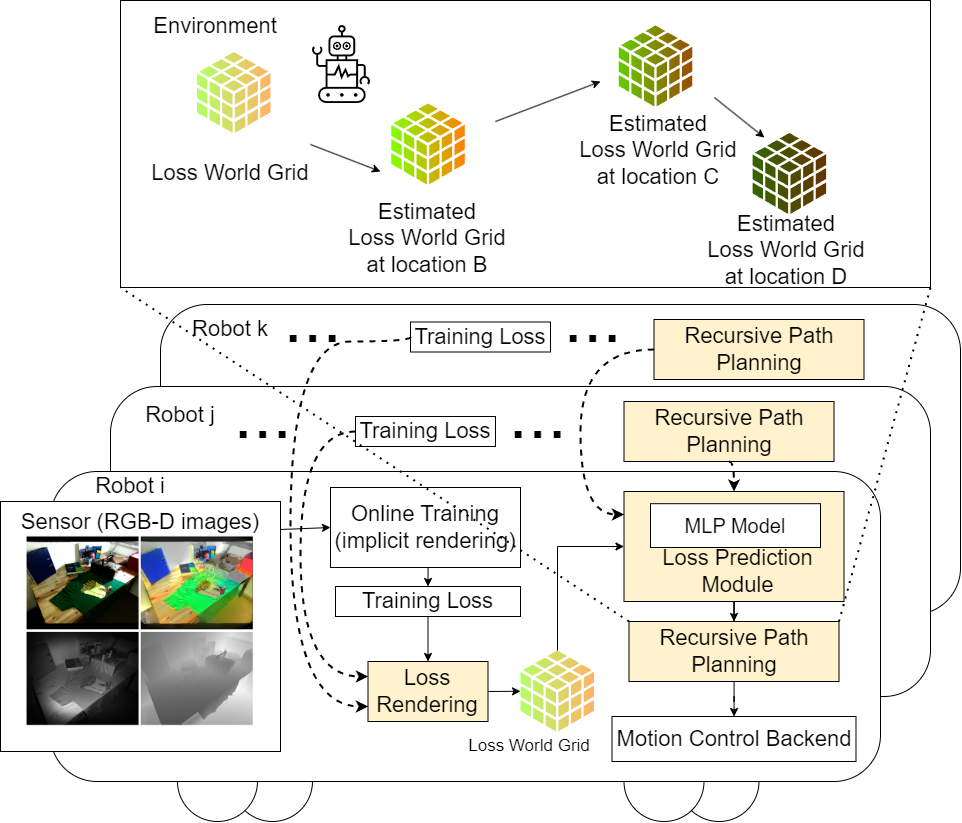
\includegraphics[width=\linewidth]{fig/overview.drawio.png}
    \caption{Overview of LODA.% During training of the online training task, training loss is exchanged and rendered to a Loss World Grid, which is used to train an MLP model that learns the loss dynamics of the Loss World Grid and is used to recursively predict the future state of the Loss World Grid in recursive path planning. The planned paths from other robots are also used to predict the future state of the Loss World Grid as the basis of local recursive path planning.
    }
    \label{fig:overview}
    \vspace{-0.5cm}
  \end{figure}


  % \begin{figure*}[t]
  %   %\vspace{-0.6cm}
  %   \centering
  %   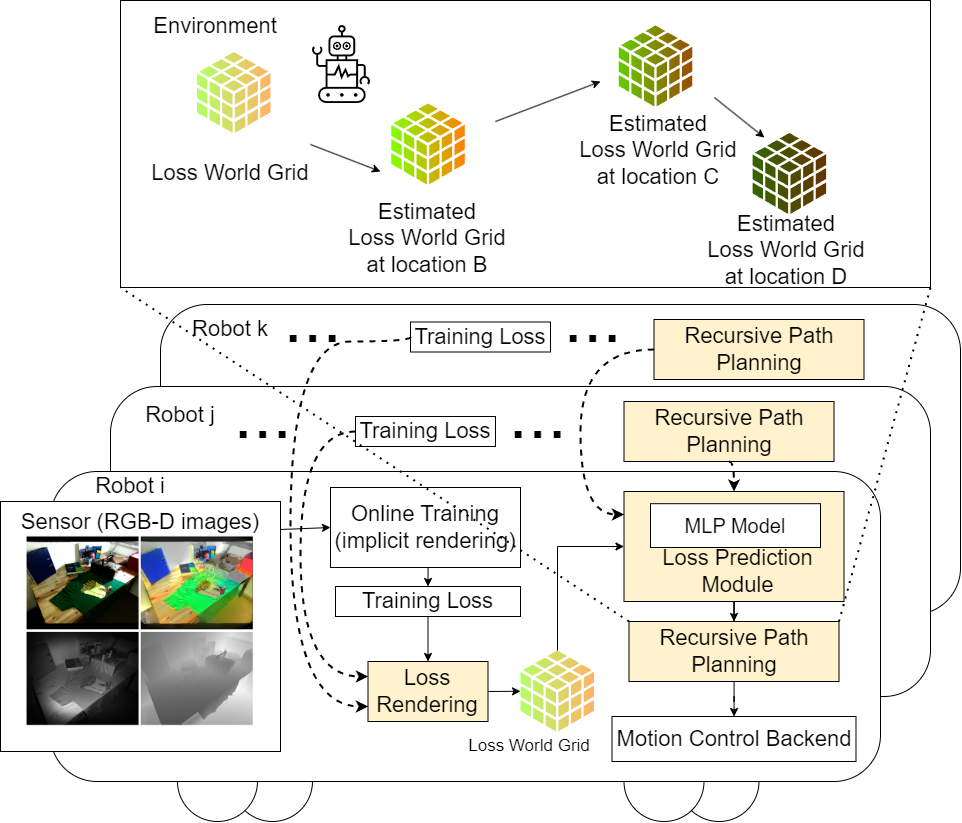
\includegraphics[width=0.98\linewidth]{fig/overview.drawio.png}
  %   \caption{New Overview of MIAS}
  %   % \label{fig:overview}
  %   %\vspace{-0.3cm}
  % \end{figure*}


% This chapter presents the architecture of LODA and gives an overview of how LODA models the loss dynamics of the environment and how it is used to search for path with optimal accumulated information gain with a single robot or the cooperation of multiple agents in the LODA-RPP algorithm.

As shown in Fig.~\ref{fig:overview}, assume that each robot is a four-wheel robot with sensors (e.g., cameras, lidar) attached to it and it is periodically taking samples ($I_i \in \bm{I}$) from the sensors as the training input for an underlying online training task (e.g., 3D reconstruction), where $i=1,2,\dots$ means the $i^{th}$ sample and $\bm{I}$ is the sample space of the environment.
We assume that the size of the environment is limited and navigable for the robot, such as a room or an office.
The underlying online training task trains an AI model $\theta$ periodically on collected training input to extract knowledge (e.g., increase in accuracy of the AI model) from the environment and $L(\theta_t, I_i)$ is the training loss function on sample $I_i$ at time $t$.
The goal of automatic high quality training data acquisition for a such scenario is 

\begin{equation}
  \begin{aligned}
    \vspace{-0.5cm}
    \mathop{\min} & \quad t, m \\
    \mathop{s.t.} & \quad L(\theta_t)\approx \frac{1}{m} \sum_{i=1}^{m} L(\theta_t, I_i) < t_{loss} \\
      & \quad C(\{I_i\}) > t_{coverage}
  \end{aligned}
  \label{mini1}
\end{equation}
where $C(\cdot)$ is the coverage estimation of the samples.
It means finding a minimum sequence of samples that fastest covers the environment and have the highest information gain to reduce the loss function which forms the navigation path of the robots.
% While the fast coverage problem is well approximated by traditional RRT algorithms, we aim at approximating the problem of finding a navigation path for the robot to acquire the sequence of ${I_i}$ of highest information gain in this paper.
% We are aiming to find a navigation path for each robot to optimize quality of the collected training data so that the online training task can achieve high performance (e.g., overall loss function $L(\theta_n)$ lower than a threshold $t$) within as short as possible time (thus as few as possible training iterations and training input): 

% \begin{equation}
  %   \begin{aligned}
    %     \mathop{\min} & \quad n, m \\
    %     \mathop{s.t.} & \quad L(\theta_n) < t \\
    %   \end{aligned}
    %   \label{mini}
    % \end{equation}
    
% The fact that $\theta_t$ is varying over time invalidates the methods that statically consider the model $\theta$ and we explore the dynamic metrics of the training model and come into loss dynamics.
Considering the evolution of $\theta$ over time, the variation of $\theta_t$ is typically impossible to predict. % and thus we we cannot extend the active learning methods to predict the future $I_{i+1}$ with highest information gain when we have predicted $I_{i}$ for the current model.
Instead, we predict the level of information gain when $I_{i}$ is acquired exploiting loss dynamics through the following components of our system: loss rendering, loss dynamics modelling and future loss prediction, and finally forms an optimal path with recursive path planning as discussed below.

\vspace{-0.5cm}
\subsection{Loss Prediction Module}
In LODA, we store the running statistics of training loss by rendering it to a sparse grid of tensor named World Loss Grid (WLG) in correspondence to the coordinates of the training samples in the environment.
An MLP model is periodically trained based on these data to learn the dynamics of loss and predict future loss given a desired sampling position and orientation.
The MLP model is online trained to adapt to possible different loss intensity and different loss dynamics in different environments or online training tasks.

% In LODA, based on the Loss Prediction Module, we predict the future training loss when the training AI model is trained on newly collected data and calculate loss reduction as an approximation of possible information gain (discussed in detail in the next section) for recursive path planning.
% To predict such loss reduction for path planning on every robot, we periodically sample and distribute the training loss among all robots.
% The loss and extra information such as its average, weight (times visited), the sampling position and orientation of the training data are then rendered and stored in a sparse grid of tensor named World Loss Grid, which is in correspondence to the environment.
% An MLP model is periodically trained based on data on the grid to predict future loss given a desired sampling position and orientation and the corresponding tensors (selected by frustum selection) on the sparse grid, which is the basis for information gain estimation.
% The MLP model is online trained to adapt to possible different loss intensity and different loss dynamics in different environments or online training tasks.

% Since this prediction of training loss from has the same meaning of the input data for prediction from the sparse grid, which is also loss, the prediction result can be merged back to the sparse grid for the prediction when searching for the next step in a recursive way.

\vspace{-0.5cm}
\subsection{Recursive Path Planning}
% Since it is impractical to search all possible paths even in an environment with limited size,
% we integrate our path planning with RRT* algorithm which searches obstacle-free paths in width-first style and recursively estimate the accumulated information gain.
As in Fig.~\ref{fig:overview}, starting from the original WLG, we predict the training loss when a next step is taken using the loss prediction module (excluded for simplicity in the figure) and incrementally render a new sparse grid,.
On the basis of the predicted new sparse grid, we continue to predict the training loss for the following steps recursively and finally at the end of the path the accumulated information gain estimation of the whole path is calculated as the difference between the final predicted sparse grid and the original to search for the path with optimal accumulated information gain.
% With the estimation results of the candidate paths, the path with the highest potential accumulated information gain can be found.

To support multi-robot cooperation in active high quality training data acquisition, a robot should consider the plans from other robots and estimate the impact of the plans from other robots for the decision making of itself.
In LODA this can be easily achieved with the above design.
We recursively predict the resulting sparse grid of training loss of planned paths from other robots and merge it with the original WLG as the basis of recursive path planning of this robot, resulting in a cooperative path considering the impact from the possible actions from other robots.




\section{Design}
% This section introduces the design of the main components and algorithms of LODA, the Loss Prediction Module and LODA-RPP algorithm in details.
\subsection{Loss Prediction Module}
\subsubsection{Loss rendering}

We assume that the sampling environment is limited (e.g., within a room or office) which can be divided into a grid of finite 3D cells ($u_k\in \bm{u}$) and there exists a correspondence relationship that $I_i = Render(\bm{u}, p_i)$ where $p_i$ is the sampling perspective (position and orientation) of $I_i$, and $\bm{u}_i$ is the set of related cells, typically regulated by depth values sensed at $p_i$ and only a fraction of $\bm{u}$ is visible which we refer to as $\bm{u}_i$.
Thus, 
$L(\theta_t)$ in Equa.~\ref{mini1} is rewritten as $L(\theta_t) \approx \sum_{i=1}^{m} L'(\theta_t, \bm{u}_i, p_i) < t_{loss}$.
% \begin{equation}
%   \begin{aligned}
%     \mathop{\min} & \quad n,m \\
%     \mathop{s.t.} & \quad L(\theta_t) \approx \sum_{i=1}^{m} L'(\theta_t, \bm{u}_i, p_i) < t_{loss} \\
%             & \quad c({I_i}) > t_{coverage}
%   \end{aligned}
%   \label{mini2}
% \end{equation}

While the fast coverage problem is well approximated by traditional RRT algorithms for a limited environment and the number of samples needed to train an AI model is typically much larger than the number of samples needed to cover the environment, thus we may consider the problem based on a set of $\{I_i\}$ that already satisfies the coverage constraint and finding new samples that reduce $\sum_{i=1}^{m} L'(\theta_n, \bm{u}, p_i)$ the most, and we define such diff as:
\begin{equation}
  \begin{aligned}
    D(i+1) &= \sum_{i=1}^{m+1} L'(\theta_t, \bm{u}_i, p_i) - \sum_{i=1}^{m+1} L'(\theta_{t+1}, \bm{u}_i, p_{i}) \\
    & = \sum_{i=1}^{m} \Delta {L'}^i_t + \Delta {L'}^{m+1}_t
  \end{aligned}
\end{equation}
where $\Delta {L'}^i_t = L'(\theta_t, \bm{u}_i, p_i) - L'(\theta_{t+1}, \bm{u}_i, p_{i})$.
We assume knowledge from $I_{m+1}$ does not conflict with the previous data, which means it will not increase loss of previous data and $\sum_{i=1}^{m} \Delta {L'}^i_t \geq 0$.
We have 
\begin{equation}
  D(i+1) \geq \Delta {L'}^{m+1}_t
  \label{delta}
\end{equation}
which means the beginning from $\theta_t$ to $\theta_{t+1}$, the training loss reduction over $\bm{u}_{m+1}$ and $p_{m+1}$ reflects the level of information gain can be learned from $I_{m+1}$.
By now we have associated the variation of training loss bounded to a set of grid cell and its sampling pose with the possible information gain, whose prediction model can be online trained using existing data as shown in the following subsection.
$p_{m+1}$ (and thus $\bm{u}_{m+1}$) maximizing such loss variation is the training data with highest information gain.

We have approximated the possible information gain of an unknown sample with the difference between the loss rendered to the visible area of a 3D grid of the environment under the regulation of sampling position and orientation and depth values.
Given a candidate $p_{m+1}$, the parameters to calculate $\Delta {L'}^{m+1}_t$, $\theta_{t+1}$ and the actual sensor input are still unknown, but their resulting loss is of low dimension and can be modelled via online training methods.
% While the required parameters to calculated $\Delta {L'}^{m+1}_t$ from a specific $p_{m+1}$
% To predict the training loss variation on the grid cells, 
In LODA, we use WLG $G$ to represent the environment, which is a four-dimensional sparse grid with the last dimension storing information for loss prediction.
Specifically, we divide the possible sampling distances and orientations to consider into different levels, $n_{dist}$ and $n_{dir}$.
When a loss value is rendered to a cell on the grid, we store the number of times that this loss is hit (weight), its average and the latest loss value together with the sampling position and orientation using position encoding.

\subsubsection{Training and inference}
Given the groundtruth loss $l_u$ of a cell, its sampling distance and orientation$i_{dist}$ and $i_{dir}$ and $G$, a three-layer MLP model $M$ is trained to learn and predict the training loss. The training loss function of $M$ is:
\begin{equation}
  L_M = \Vert M(i_{dist}, i_{dir}, G_{j,k,h}) - l_u \Vert_2
\end{equation}
which means modelling the dynamics (or varying trend) of loss of a cell based on history information.
During inference, given a sampling pose $p$, we calculate the visible cells $\bm{u}_p$ and the sampling distance and orientation of each cell. For a cell $u$ on the WLG sampled at $i_{dist}$ and $i_{dir}$, its loss is predicted as $l_u = M(i_{dist}, i_{dir}, u)$.
Note the inference input and inference result of $\bm{u}_p$ together are of the same form of information needed to render cells for $G$, forming the basis of the recursive path planning in LODA-RPP algorithm.


\subsection{LODA-RPP Algorithm}
In LODA, candidate paths (sequences of sampling poses.) are generated by random sampling algorithms such as RRT. 
While traditional active learning methods can only consider the information gain of one pose in a path, we manage to calculate the accumulated information gain along the path with LODA-RPP to get a better estimation of overall information gain, and finally find the optimal path with highest accumulated information gain.

\begin{algorithm}[h]
  \caption{Recursive State Prediction.}
  \label{alg:rsp}
  \KwIn{WLG: $G$; Loss Prediction Module with MLP: $M$; candidate path: $P$}
  \KwOut{predicted future state of World Los Grid when candidate path is executed: $G'$}
  \BlankLine
  \uIf{len($P$) = 0}{return $G$} 

  $p$ = $P$[0];

  $\bm{u}_p$, $\bm{i}_{dist}$, $\bm{i}_{dir}$ = FrustumCalculation($p$);

  $l_{\bm{u}_p}$ = $M$($\bm{i}_{dist}$, $\bm{i}_{dir}$, $\bm{u}_p$);

  $G_p'$ = LossRendering($l_{\bm{u}_p}$, $p$, $G$);

  $G_{next}$ = overwrite $G$ with $G_p'$;

  $P_{next}$ = $P$[1:];

  $G'$ = RecursiveStatePrediction($G_{next}$, $M$, $P_{next}$);
\end{algorithm}

We first introduce the process of Recursive State Prediction as shown in Alg.~\ref{alg:rsp}.
With the WLG $G$ and MLP model $M$, given desired sampling pose $p$ from a path $P$,
We first compute the visible cells $\bm{u}_p$ on $G$ and their sampling distances and orientations, with which we can predict their future training loss $l_{\bm{u}_p}$ from $G$.
We then use the prediction result $l_{\bm{u}_p}$ and sampling pose $p$ to render cells in $\bm{u}_p$ as a partial update of $G$, referred to as $G_p'$, which is the predicted future state of $\bm{u}_p$ in $G$ when the robot navigates to $p$ to acquire new training input.
Merging $G$ and $G_p'$, we will get the predicted WLG when we have arrived at $p$ and taken samples.
Recursing such process, we will get the future WLG when every step in $P$ is taken.

\vspace{-0.3cm}
\begin{algorithm}[h]
  \caption{Framework of LODA-RPP algorithm}
  \label{rpp}
  \KwIn{WLG: $G$; Loss Prediction Module with MLP: $M$; start pose: $p$; planned paths from other robots: $\bm{P}_o$}
  \KwOut{Planned Path: $P$}
  \BlankLine
  \For{$P'$ in $\bm{P}_o$}{$G$ = RecursiveStatePrediction($G$, $M$, $P'$);}

  generate candidate paths $P_{candidate}$;

  $e$ = 0;

  $P$ = [$p$];

  \For{$P'$ in $P_{candidate}$}{
    $G'$ = RecursiveStatePrediction($G$, $M$, $P'$);

    $e'$ = $G$ - $G'$;

    \uIf{$e'$ > $e$}{$P$ = $P'$}
  }
\end{algorithm}
\vspace{-0.3cm}

Integrating Recursive State Prediction, LODA Recursive Path Planning (LODA-RPP) in Alg.~\ref{rpp} is able to predict the accumulated information gain of each candidate path.
First, we update the WLG temporarily with the planned paths from other robots using Recursive State Prediction to consider their impact on the path planning of this robot to search for cooperative paths.
Then for every candidate path, we estimate the accumulated information gain of each path by predicting their resulting WLG when poses in each path are executed with Recursive State Prediction and computing the difference between the starting WLG and resulting WLG.
Finally the outputted path is the optimal path with highest estimated accumulated information gain which also cooperates with other robots.

\section{Implementation}

We implemented LODA based on Robot Operation System 2 (ROS2) Galactic, Python3.8 and PyTorch on Ubuntu20.04, using the default navigation stack of ROS2.
We maintained the Loss World Grid on a sparse coordinated tensor using PyTorch, instead of a dense tensor, because in a room there are typically a lot of empty space that holds no useful information and will not have loss being computed.
This design significantly reduces the memory and computation burden.
% The sparse coordinated tensor of PyTorch currently only supports index selection along one dimension, which is inconvenient for computation over the 4 dimensional Loss World Grid.
% Thus we created a flattening interface that stores the Loss World Grid as a two dimensional sparse tensor and coverts multi-dimensional indexing over the Loss World Grid to one dimensional indexing, so as to support efficient analysis and computation over the Loss World Grid.
% To support slicing and index selection in the Loss World Grid that is compulsory for enquiry of features from the Loss World Grid and compute partial updates of it, we virtually 

% LODA on one robot communicates with the underlying online training task and other robots via the ROS2 interface.
% Using the Data Distribution Service of ROS2, LODA and the underlying online training task run on different processes avoiding the performance bottleneck of GIL of Python and can exchange the planned paths and training loss with each other and other robots needless to explicitly handle the network connections between them.
% We use the default navigation stack of ROS2, Nav2, which is responsible to find and mark navigable places based on sensor input and execute the planned path step by step, while avoiding obstacles.

\section{Evaluation}
\subsection{Evaluation Settings}

\subsubsection{Testbed}
For reproducibility and stability, we evaluated LODA over a server with 4 2080Ti 11GB GPUs, an Intel(R) Xeon(R) Silver 4116 2.10GHz CPU and 128 GB RAM.
When extending the number of robots involved, each robot is allocated a unique GPU to avoid performance bottleneck due to sharing GPU.


\subsubsection{Workload}
We choose a state-of-the-art implicit rendering method, BNV Fusion~\cite{li2022bnvfusion} as our workload, which reconstructs dense 3D mesh of the environment based on a sequence of depth images and their sampling poses.
BNV Fusion~\cite{li2022bnvfusion} is composed of a sparse grid of latent codes which is an implicit representation of the 3D environment and a pre-trained decoder.
% Given a depth image and its sampling pose, BNV Fusion predict a depth image corresponding to the sampling pose by decoding the latent codes using the decoder, compute mean square error between the predicted depth image and the input one as the loss and optimize the latent codes, forming an online training pipeline.
We use 2cm voxel size in BNV Fusion, other default hyper-parameters and the default decoder parameter checkpoint officially released.

% To support distributed training when the number of robots involved increases, we implemented ROG~\cite{guan_rog_2022} as the parameter synchronization backend which removes the parameter update synchronization barrier among the robots (robots do not need to synchronize parameter updates on every optimization step), enables partial parameter synchronization that has most contribution to performance of the AI model while ensuring convergence.
% The voxel size (proportional to the size of the local geometry for a local latent code) for the single 3D objects is 1cm to extract finer details and the voxel size for the Replica dataset is 2cm to save GPU memory and map a large scene.
% We also use the default hyper-parameters in its demo setting and use their released checkpoint for the encoder and the decoder.
% It is notable that the latent codes $\theta$ are only trained for 10 iterations on an NBV $v_{n+1}$ being input to $\bm{v_n}$ in BNV Fusion.


\subsubsection{Dataset}
We use the Habitat simulator~\cite{szot2021habitat} and Replica dataset~\cite{straub_replica_2019} commonly used in computer vision tasks. 
% The Habitat simulator renders high quality 3D scenes from the Replica dataset and simulates realistic physical trajectory of simulated agents in the 3D scene in real time and we ported it with the ROS stack by publishing its simulated output, including RGBD images and the poses of the simulated agents using the DDS of ROS.
We select three real-life high quality scenes from the Replica dataset of three levels of sizes: office\_0 sized 22.04$m^2$, hotel\_0 sized 35.88$m^2$ and frl\_apartment\_1 sized 93.10$m^2$, referred to as the small scene, the medium scene and the large scene.
The robots are spawned at random positions in the scenes.

The Habitat simulator broadcasts the simulated rgb samples of each robot at 10 Hz, and the online training task of BNV Fusion collects and processes the simulated output to optimize the training model at 1 Hz.
Every 2 minutes a reconstructed dense 3D mesh of the scene is produced to estimate the model's performance.


\subsubsection{Baselines}
We choose two state of the art active learning methods as our major baselines, namely Badge~\cite{ash_deep_2020} and ActiveNerf~\cite{avidan_activenerf_2022}.
Badge~\cite{ash_deep_2020} (referred to as badge) estimates the information gain of a possible input by computing the gradient magnitude and diversity with respect to parameters in the final (output) layer, which is computed using the most likely output according to the model.
% The diversity is measured by comparing the direction of the gradients with those of the existing input.
% And the one with highest magnitude and diversity is considered the most informative.
ActiveNerf~\cite{avidan_activenerf_2022} (referred to as uncertainty) is a method optimized for implicit rendering that models the training model output as a Gaussian distribution and add an extra model head that learns to predict the output variance as a measurement of uncertainty, where the zones with highest uncertainty is considered of highest information gain.
% They are both able to find the possible training input with highest information gain for the current training AI model, but would fail to provide a navigation path with highest accumulated information gain without considering the evolution of training AI model along the acquisition path.
To extend them to multiple robots, we duplicate these methods on each robot.
The baselines all use the same navigation stack as our system, with RRT* algorithm providing candidate training input for them to select from.


\subsubsection{Metrics}
To estimate the quality of the reconstructed mesh, we choose the completion ratio that is commonly used in 3D reconstruction tasks~\cite{li2022bnvfusion,zhu_nice-slam_2022}.
To calculate completion ratio, starting from vertices in the groundtruth mesh, we query for vertices in the reconstructed mesh whose distance is within a threshold and the ratio of successful query is the completion ratio, which reflects how close that the reconstructed mesh is to the groundtruth.
We also used Structure Similarity Index Measure (SSIM) to estimate the similarity between consecutive samples in breakdown to show how LODA instructs the robot to collect training input with higher diversity and quality.
SSIM close to 1 means that the two estimated images are identical, and SSIM smaller means less similar.


\subsection{End-to-End Performance}
\subsubsection{Different Sizes of Scenes}
\begin{figure*}[h!]
\centering
\vspace{-0.9cm}
\subfloat[office\_0 (Small Scene)]{
    \label{fig:single_small}
    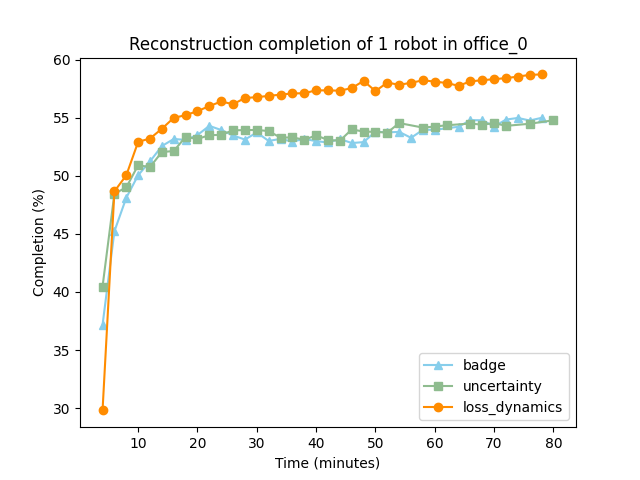
\includegraphics[scale=0.35]{fig/single/1_completions_plot_office_0.png}}   
\subfloat[hotel\_0 (Medium Scene)]{
    \label{fig:single_medium}
    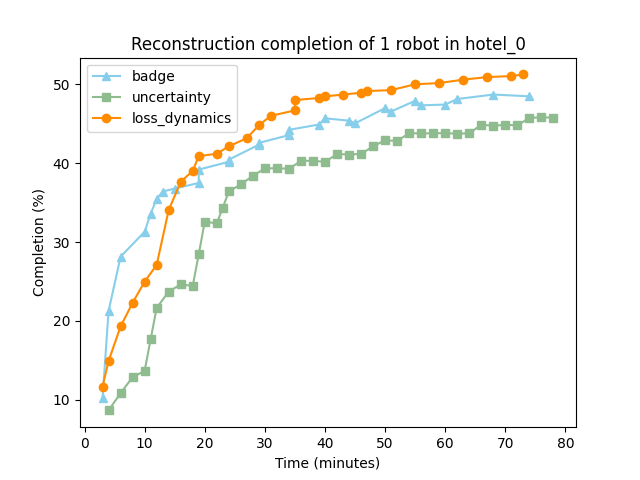
\includegraphics[scale=0.35]{fig/single/1_completions_plot_hotel_0.png}}
\subfloat[frl\_apartment\_1 (Large Scene)]{
    \label{fig:single_large}
    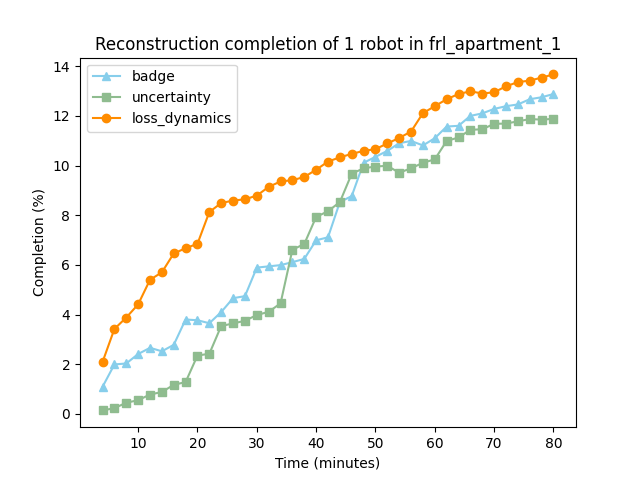
\includegraphics[scale=0.35]{fig/single/1_completions_plot_frl_apartment_1.png}}
\vspace{-0.3cm}
\caption{The completion ratio of the reconstructed mesh with one single robot in different sizes of scenes.}
\label{fig:single_robot}
\end{figure*}

We first compare the performance of three different methods (LODA referred to as loss\_dynamics in the figures) with one robot exploring and acquiring training data according to their information gain for the 3D reconstruction process in scenes of different sizes.
Note that the visible area of the whole scene to the four-wheel robot is limited because of the comparatively low perspective of a robot, the completion ratio in each scene is limited and lower than one hundred percent.

The experimental result in Fig~\ref{fig:single_robot} shows that our method outperforms the baselines across different scene sizes in terms of both time to reach the same completion ratio and the final completion ratio.
Compared with badge and uncertainty, LODA saved the time by about 43.8\% and 45.6\% for reconstruction completion ratio reaching 54\% in the office\_0 case,  by 21.5\% and 44.6\% for the completion ratio reaching 45\% in the hotel\_0 case and by 49.0\% and 49.8\% for the completion ratio reaching 8\% in the frl\_apartment\_1 scene
This can be attributed to LODA's ability to model the accumulated information gain of the whole navigation path and find the navigation path with highest accumulated information gain using the Loss Prediction Module and LODA-RRT algorithm.
% Figure \ref{fig:single_robot} illustrates the speeds at which one single robot, utilizing different active
% learning methods, reconstruct the mesh from the 3D scene with different sizes. 
% All three different sized scenes(small: Figure\ref{fig:single_small}, medium: Figure\ref{fig:single_medium}, and large: Figure\ref{fig:single_large}) prove that the advantage on reconstruction speed (xxx\% to xxx\%) of our method compared with two baselines remains, which can be attributed to the estimation of accumulated information gain along the whole candidate path with the LODA-RRT algorithm. 

Also, thanks to higher quality of training input sampled in LODA, the final completion ratio with LODA also increased across all the scenes.
Specifically, compared with badge and uncertainty, LODA achieved 4.1\% and 4.0\% higher completion ratio in the office\_0 case, 1.8\% and 6.7\% higher completion ratio in the hotel\_0 case and 1.1\% and 2.0\% higher completion ratio in the frl\_apartment\_0.

% Additionally, from Figure\ref{fig:single_small}, we can find that ours method achieve higher degree of completion (xxx\%) when our method and two baselines converge. 
% Such higher ceiling on completion degree shows that our method have the potential to reconstruct the mesh with higher quality compared with othger baselines.
% This is because baselines are viewing the training AI model in a static perspective. 
% As online training of the AI model proceeds, the parameters of the AI model keeps evolving and the possible training data of highest quality is also changed.
% In this way, baselines are unable to collect the training data of highest quality along the navigation path, leading to low quality of training data and lower quality of reconstruction.

\subsubsection{Different Numbers of Robots}

\begin{figure*}[h!]
    \centering
    \vspace{-0.8cm}
    \subfloat[office\_0 (Small Scene)]{
        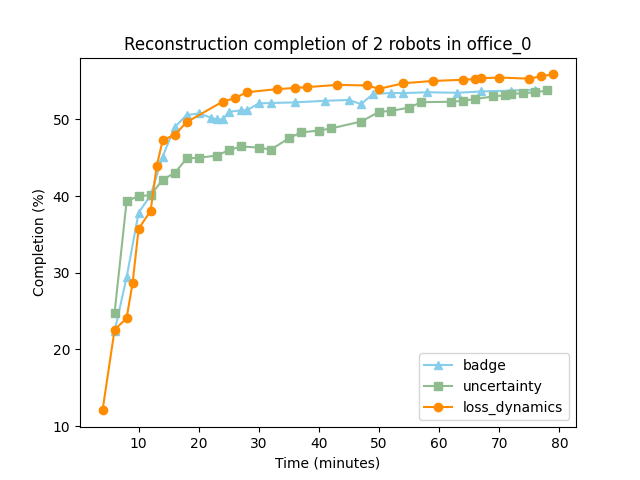
\includegraphics[scale=0.35]{fig/two/2_completions_plot_office_0.png}}   
    \subfloat[hotel\_0 (Medium Scene)]{
        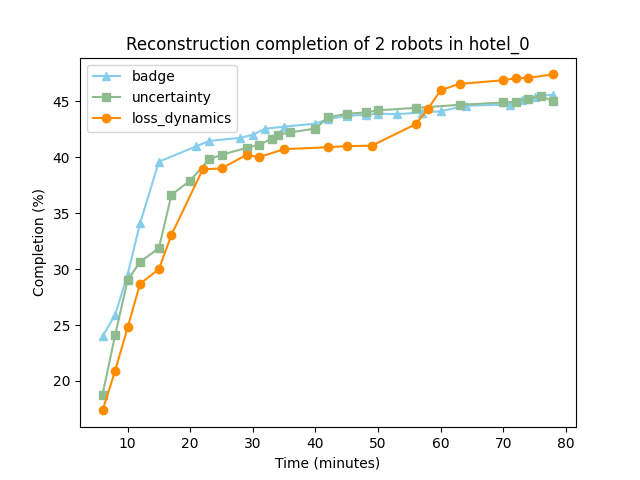
\includegraphics[scale=0.35]{fig/two/2_completions_plot_hotel_0.png}}
    \subfloat[frl\_apartment\_1 (Large Scene)]{
        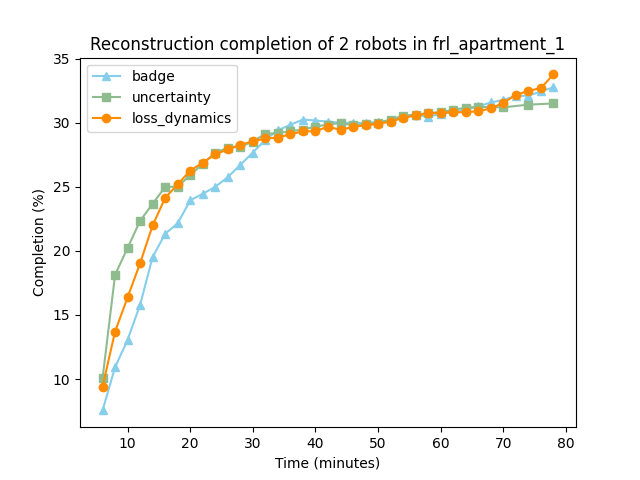
\includegraphics[scale=0.35]{fig/two/2_completions_plot_frl_apartment_1.png}}
    \vspace{-0.3cm}
    \caption{The completion ratio of the reconstructed mesh with two robots in different sizes of scenes. }
    \vspace{-0.1cm}
    \label{fig:two_robot}
\end{figure*}

We also carried out experiments of two robots exploring and taking training data in the same scenes.
And we found LODA still had the advantages of higher final reconstruction completion ratio:
compared with badge and uncertainty, LODA achieved 0.9\% and 1.0\% higher completion ratio in the office\_0 case, 1.7\% and 1.9\% higher completion ratio in the hotel\_0 case and 0.7\% and 2.5\% higher completion ratio in the frl\_apartment\_0.
But it can also be observed that the intensity of this advantages shrunk and the time to reach the same completion ratio was not evident.
This can be due to that while the baseline methods with a single robot tend to sample similar training input of low quality, duplicating them into multiple robots does extend their searching spaces for training data of high information gain and results in more diverse samples, mitigating their limitation and limiting LODA's advantages.
Nevertheless, the advantages in final completion ratio still reveal the contribution of the higher quality training data collected under the instruction of LODA.


% The experimental result shows that our method outperforms other baselines across different settings of robot number. 
% Figure X presents the training accuracy curves for different numbers of robots. 
% Under settings with 1, 2, and 3 robots, our method achieves higher accuracy than the baseline throughout the training process. 
% As the number of robots increases, the improvement in accuracy compared to the badge method further amplifies (from XX to XX). 
% This can be attributed to...  Additionally, at training times of XX, XX, and XX, our method exhibits a notable increase in accuracy growth, which can be attributed to ...

% figures: y accuracy; x time;
%  1 robot; 2 robots; 3 robots

%  fact

% ours all better than the baselines; more robot, diff larger
% badge, uncertainty > random, but due to ...
% with our system, ...

\subsection{Breakdown}

\begin{figure}[h!]
    \centering
    \vspace{-0.3cm}
    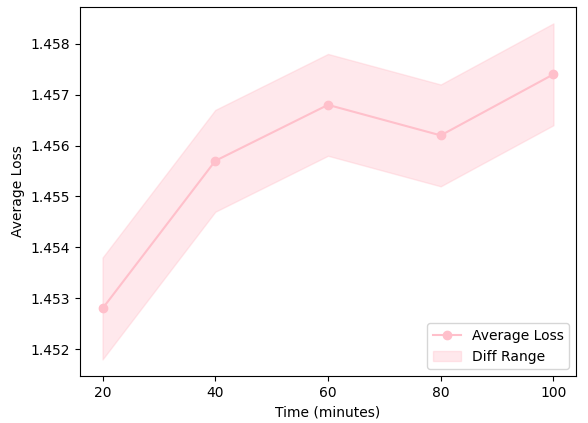
\includegraphics[width=0.7\linewidth]{fig/breakdown_prediction.png}
    \vspace{-0.3cm}
    \caption{Varying range of predicted loss and the actual loss.}
    \label{prediction}
    % \vspace{-0.5cm}
\end{figure}


In this section we inspect certain runtime statistics to better understand how LODA manages to acquire training data of higher quality.
First, we sampled and evaluated a test set sized 2000 for the Loss Prediction Module at each time spot indicated on Fig.~\ref*{prediction} in the one robot with office\_0 case and calculated the variation percentage $percent$ between the predicted loss $l_p$ and the groundtruth $l$ as $percent = \frac{\vert l_{p }- l \vert}{l}$.
The average of the variation percentage is recorded to be 1.84\% and the resulting variation range is depicted in Fig.~\ref{prediction}, which proves the effectiveness of the Loss Prediction Module.
% The average of the variation percentage is recorded to be 1.84\% and the resulting variation range is depicted in Fig.~\ref{prediction}, which proves the effectiveness of the Loss Prediction Module in modelling the loss dynamics and predicting future training loss based on rendered history of training loss from the Loss World Grid.
% This serves as a solid basis of the successive module of recursive path planning to estimate the accumulated information gain of paths and finding paths with optimal accumulated information gain.


\begin{figure}[h!]
    \centering
    \vspace{-0.3cm}
    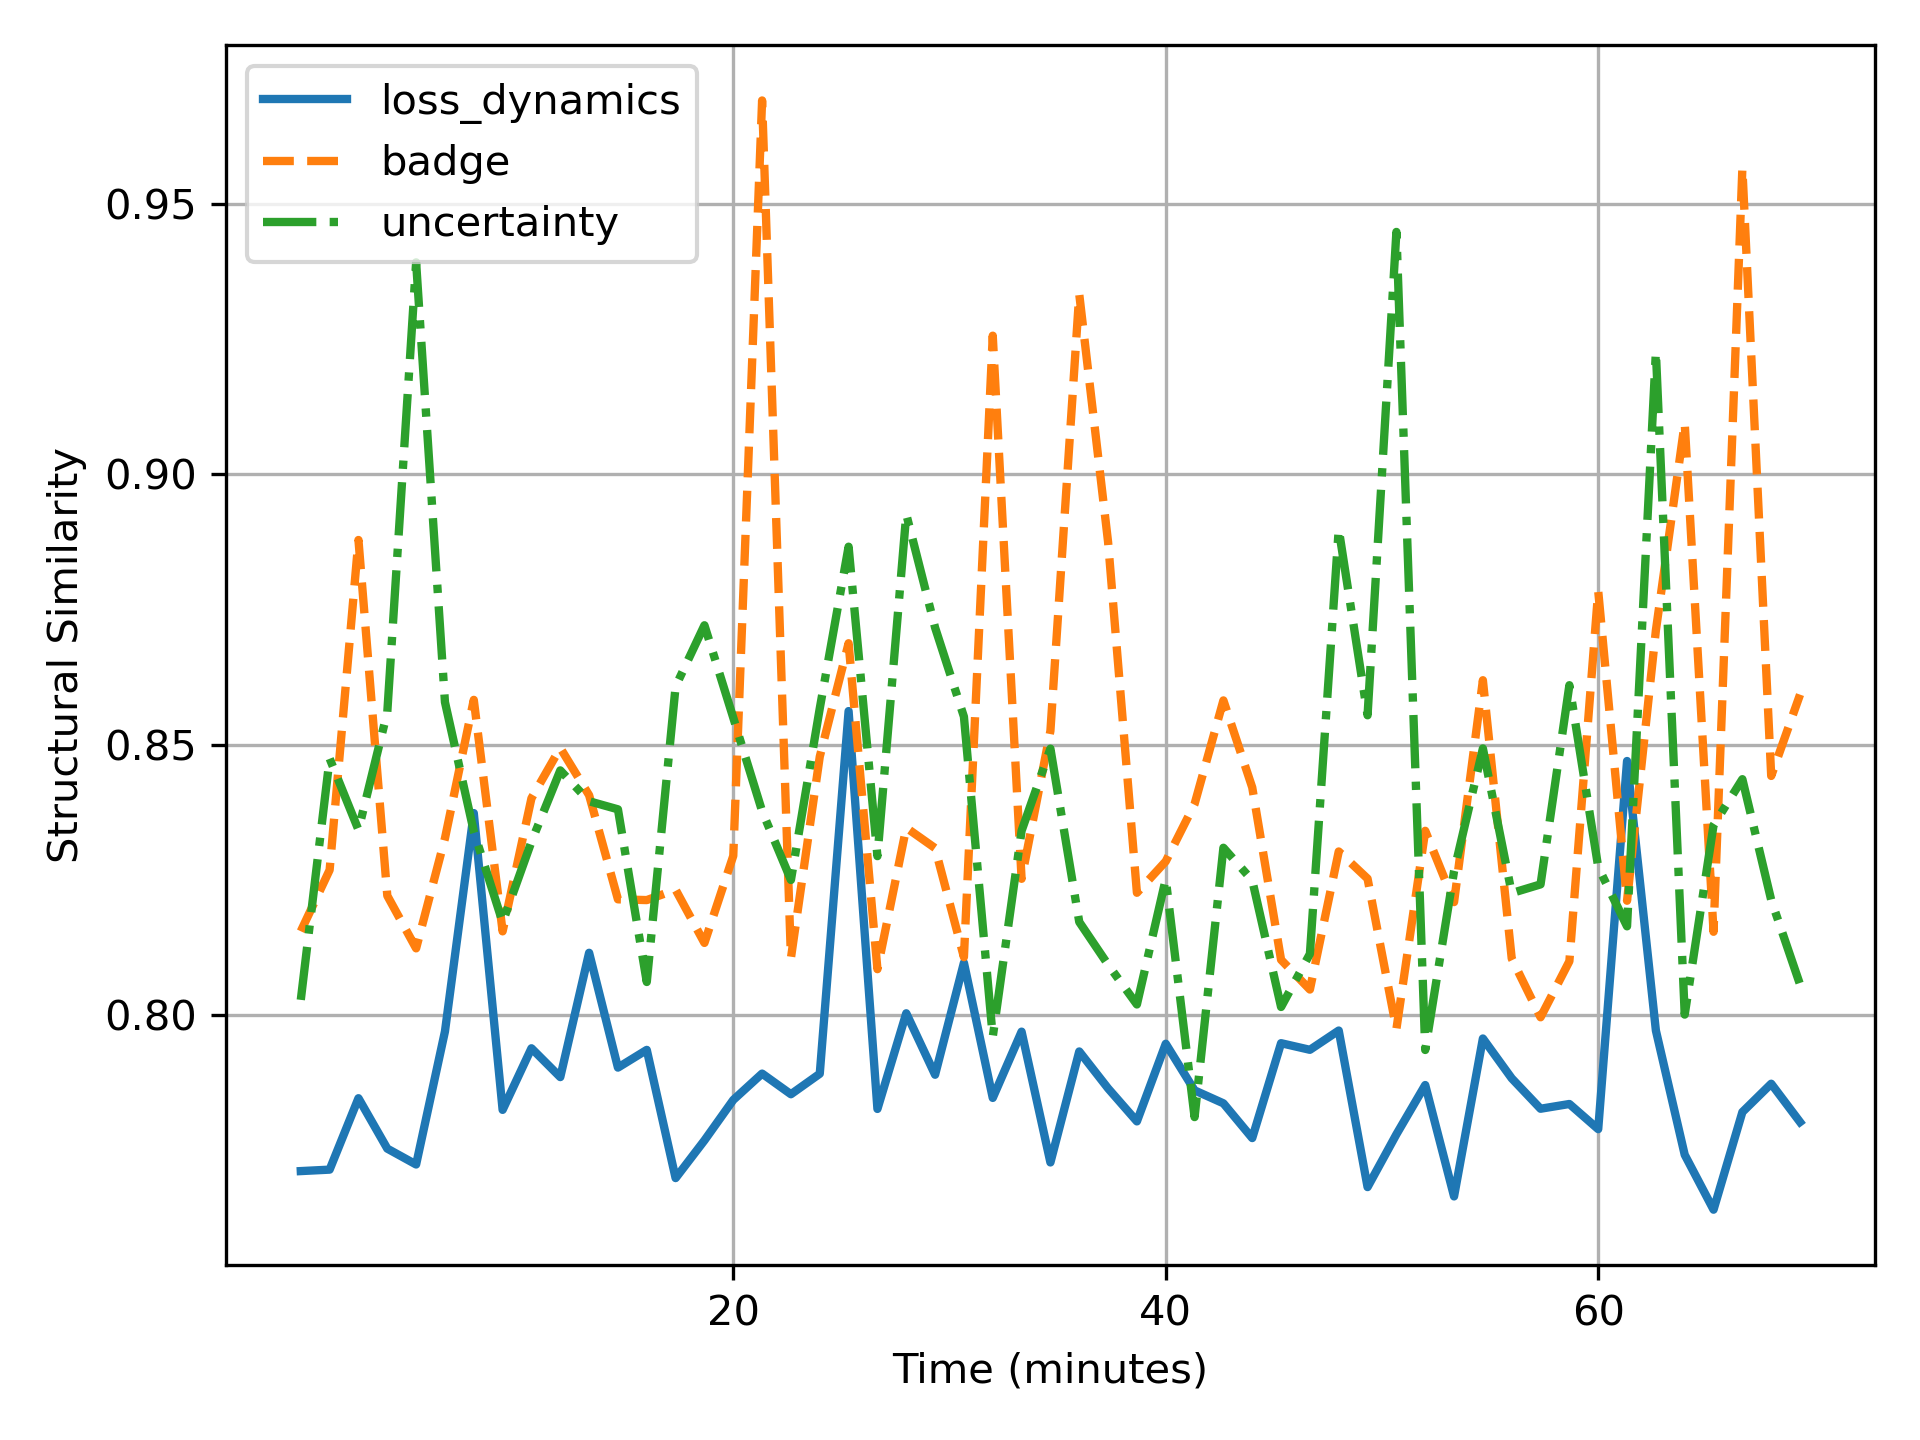
\includegraphics[width=0.7\linewidth]{fig/breakdown_similarity.png}
    \vspace{-0.5cm}
    \caption{SSIM between consecutive collected training data.}
    \label{similarity}
    \vspace{-0.7cm}
\end{figure}

\begin{table}[h!]
    \begin{center}
    \vspace{-0.3cm}
      \caption{Average SSIM between consecutively collected samples.}
    \vspace{-0.4cm}
      \begin{tabular}{c|c|c|c} % <-- Alignments: 1st column left, 2nd middle and 3rd right, with vertical lines in between
        \textbf{Methods} & loss\_dynamics & badge & uncertainty \\
        \hline
        \textbf{SSIM} & 0.789 & 0.843 & 0.840
        \label{table:similarity}
      \end{tabular}
    \end{center}
    \vspace{-0.3cm}
  \end{table}

Second, we calculated the SSIM values between depth images consecutively sampled across all evaluated methods in the  one robot with office\_0 case depicted in Fig.~\ref{similarity}, with average shown in Table.~\ref{table:similarity}.
We can learn that the baselines typically control the robot sampling depth images that are more similar than those collected under LODA.
% The recorded average SSIM is shown in Table.~\ref{table:similarity}.
Although lower SSIM does not directly translate into higher information gain between consecutive samples, higher SSIM does reveal the problem of the baselines that they tend to sample similar depth images when executing the planned path due to their static perspective of the training AI model.
% This also shows that LODA tends to control the robot to sample less similar samples under the instruction of the estimation of accumulated information gain along the candidate paths.




% \subsection{Discussion}
\section{Conclusion}
In this paper, we propose a novel dynamic perspective that models the evolution of AI model in robotic online training tasks and its influence on the information gain estimation of a navigation path with loss dynamics.
And we propose LOss-Dynamics-Aware multi-agent cooperative active sampling system for robotic online training (LODA).
Using the Loss Prediction Module and the Recursive Path Planning algorithm of LODA, we manage to model the accumulated information gain along each step of a navigation path and find the most informative path for the training AI model, which accelerates the increase of its performance.
LODA will nurture the development of more real-world robotic online training applications and improving their performance by enabling efficient and high performance automatic high quality training data acquisition.

% \newpage
\bibliographystyle{ACM-Reference-Format}
\bibliography{acmart}
\end{document}
\endinput

%%
%% End of file `sample-sigconf.tex'.
